\chapter{Applicazione mobile}

\begin{figure}[htp]
    \centering  
    \subfloat[Login]{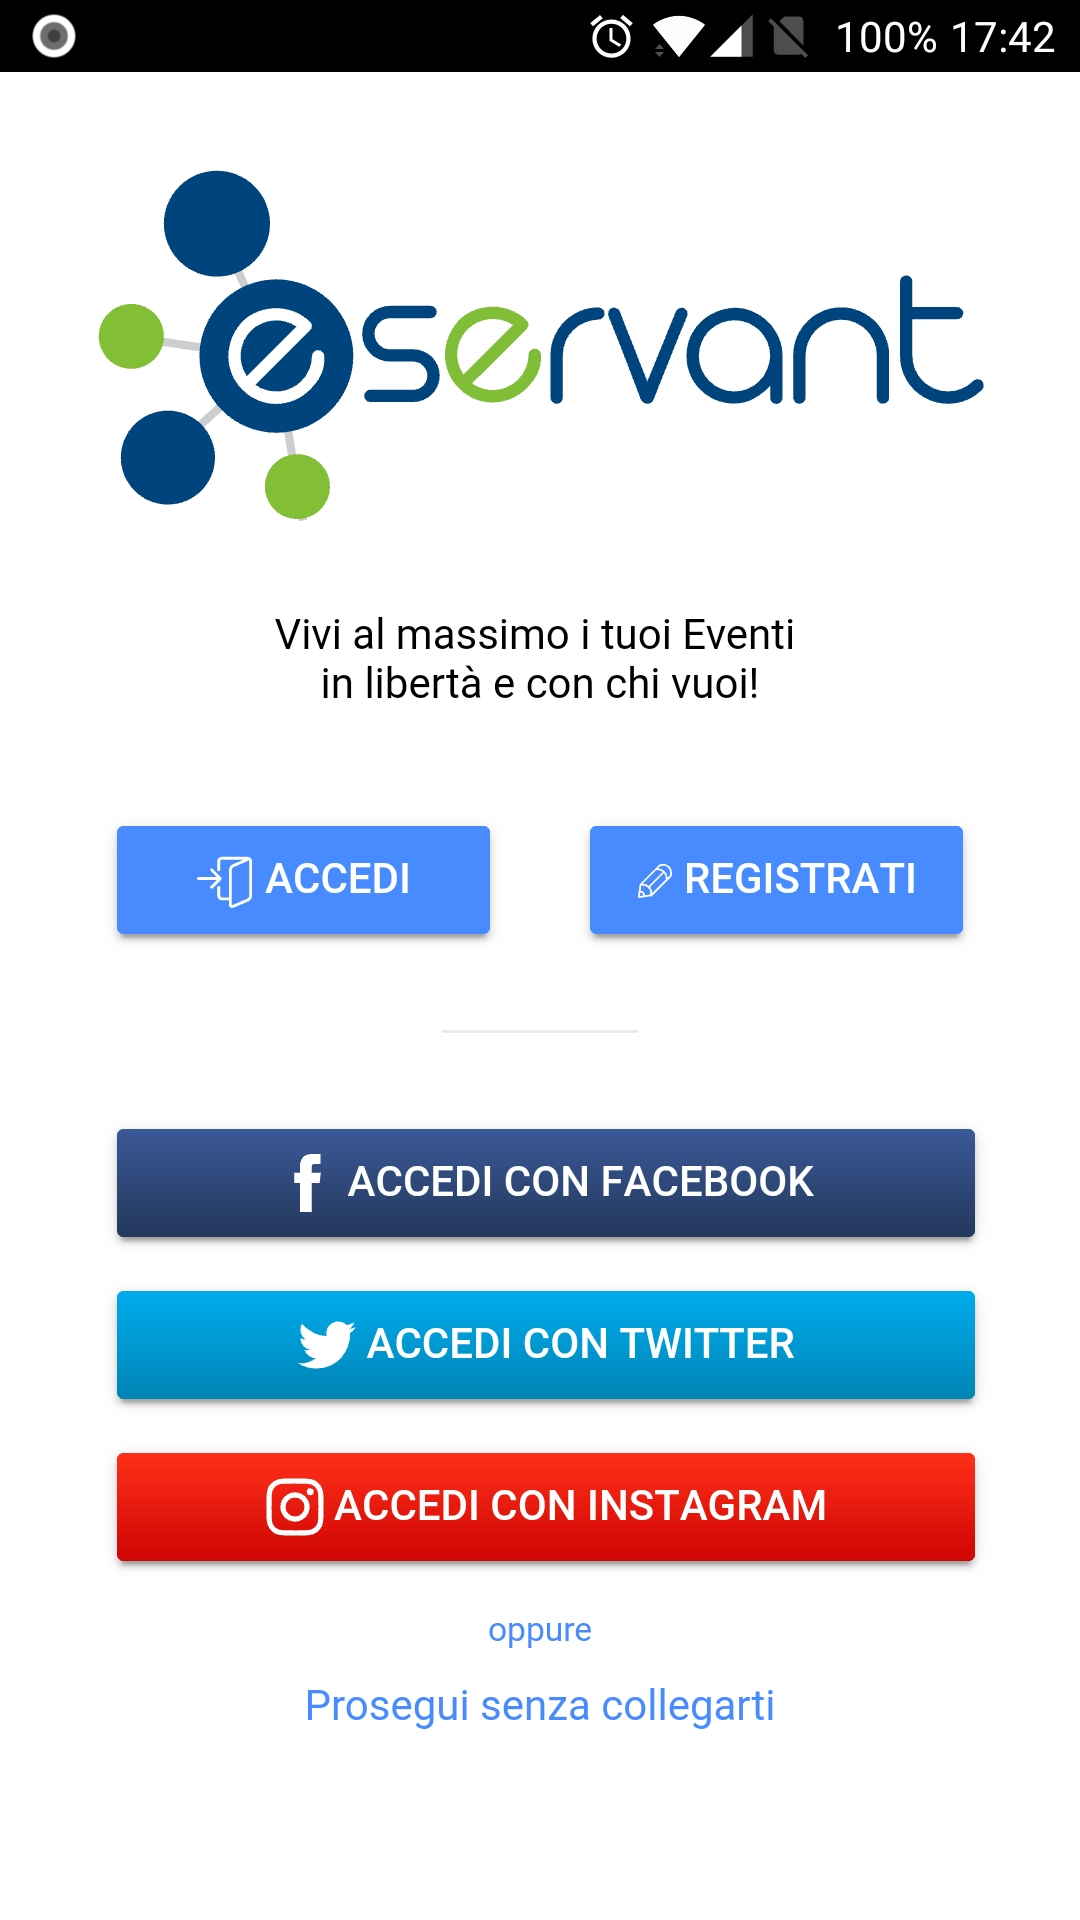
\includegraphics[scale=0.15]{img/cap2/1}}
    \subfloat[Home]{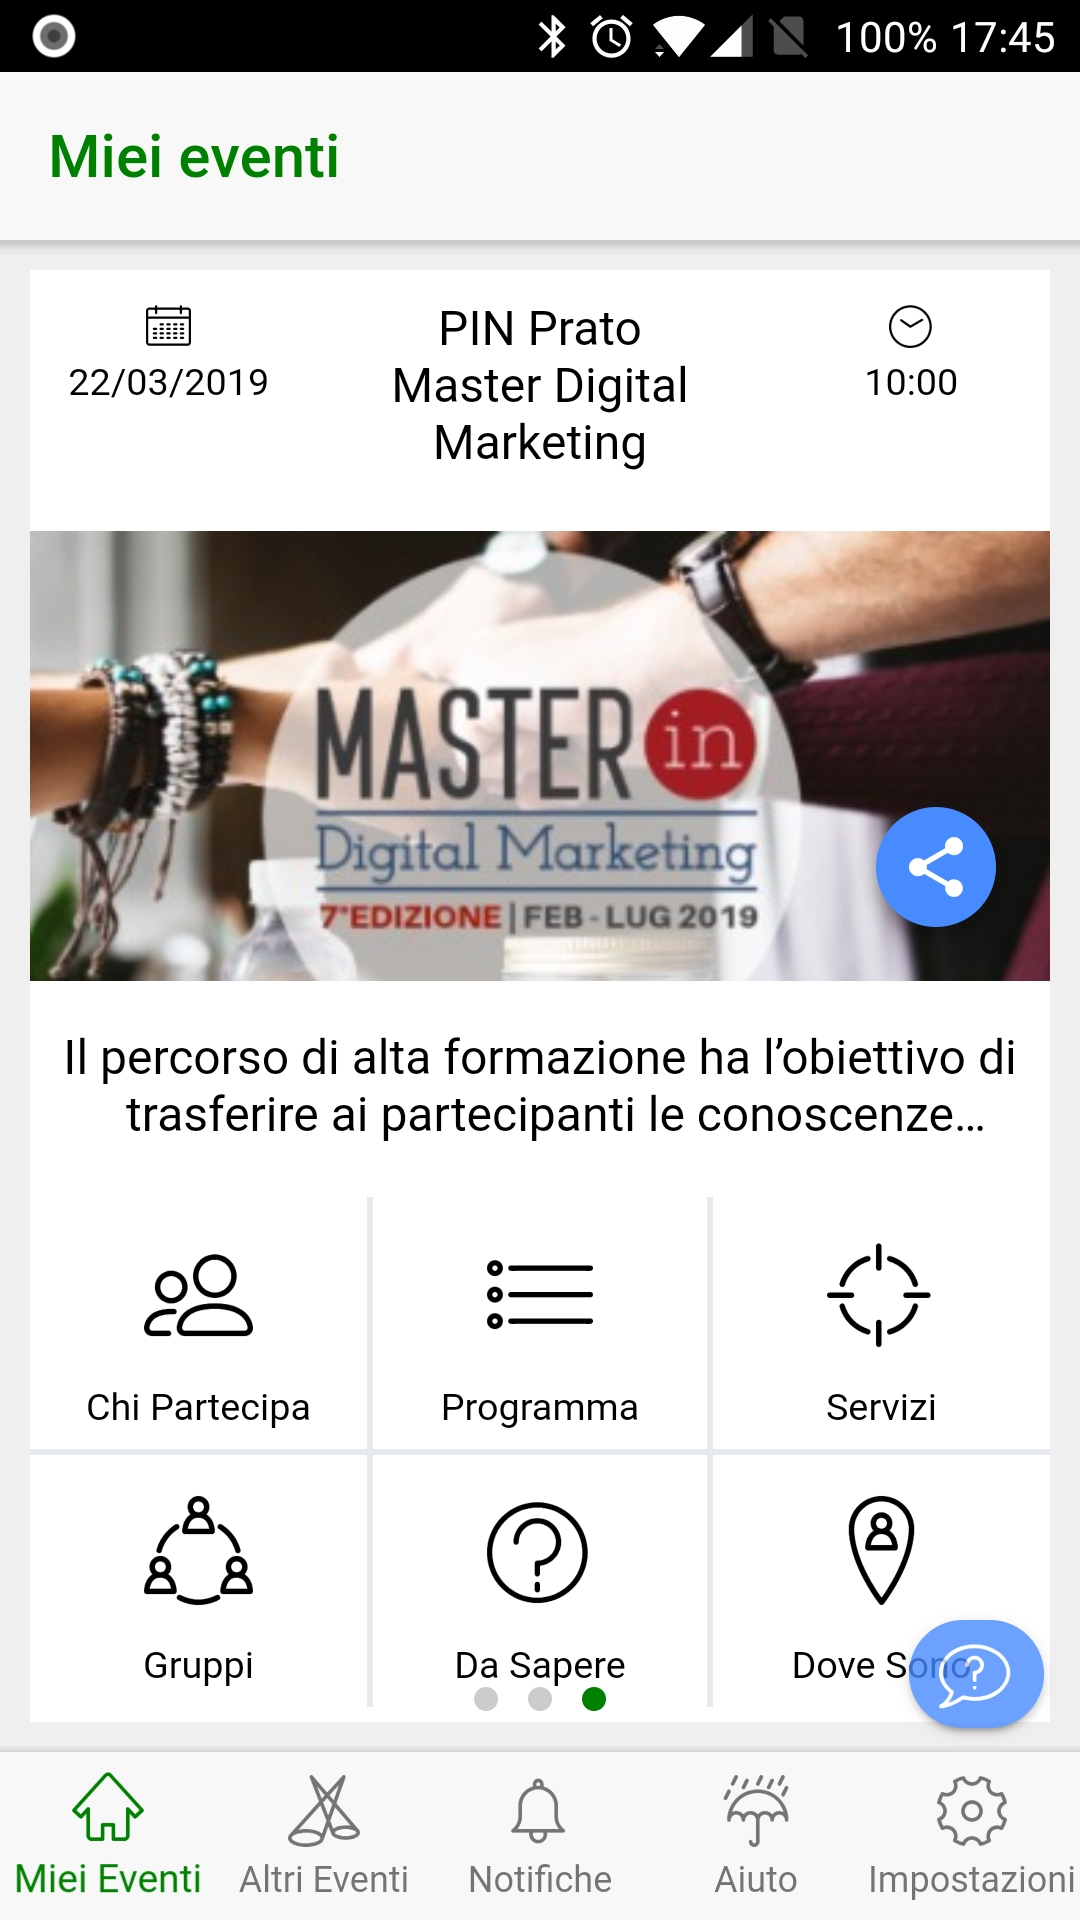
\includegraphics[scale=0.15]{img/cap2/2}}
\end{figure}

\paragraph{}
L’interfaccia della piattaforma eSERVANT verso gli utenti finali è come da progetto una APP per mobile.
Per questo insieme a Sintra Consulting s.r.l. siamo andati a disegnare in modo molto avanzato tutte le interfacce andando a quadrare requisiti di sistema/casi di uso con mockup montati all’interno di una vera e proprio demo dell’APP finale attesa.
Tale strumento ci ha permesso di valutare non solo la user experience degli utenti, ma anche di poter fornire agli sviluppatori uno strumento specifico sul quale andare a traguardare la loro attività.

Il prototipo di APP è quindi stato creato andando a realizzare slide sui cinque temi di fondo:
\begin{itemize}
\item presentazione e riconoscimento
\item gestione evento e socialità
\item gestione delle funzioni di aiuto
\item gestione delle funzioni di mobilità
\item gestione delle funzioni di navigabilità e mappe
\item gestione del proprio profilo
\end{itemize}

\section{Framework Ionic}
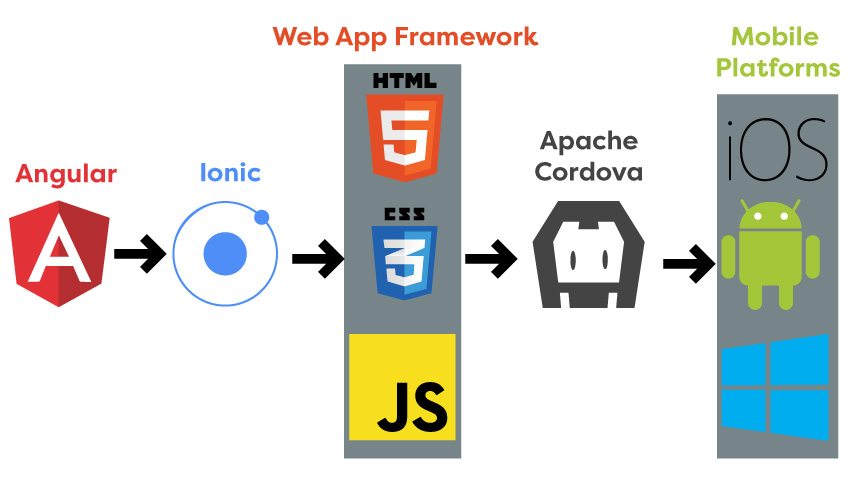
\includegraphics[scale=0.50]{img/cap2/angular-ionic}\\
Ionic è un HTML5 SDK lanciato nella sua prima versione nel 2013 e progettato per essere la base per lo sviluppo di app mobili ibride. 
Sviluppare un app mobile ibrida significa scrivere un unico code base per i due OS più famosi: IOS e Android.

Ionic viene distribuito come pacchetto installabile con npm, il package manager di Nodejs.
Node.js è un ambiente di run-time JavaScript open-source e multipiattaforma che esegue codice JavaScript all'esterno di un browser, lato server per esempio.

Installazione Ionic tramite CLI Linux
\begin{lstlisting}
npm install -g ionic
\end{lstlisting}

Elementi positivi emersi sviluppando in Ionic:
\begin{itemize}
    \item essendo tra i più famosi web framework, la \textbf{velocità di sviluppo} è un aspetto caratterizzante di Ionic
    \item \textbf{semplice} da capire
    \item supporta il \textbf{live reload} permettendo così al developer di vedere immediatamente le modifiche direttamente sul dispositivo mobile
\end{itemize}
    
Elementi negativi emersi:
\begin{itemize}
    \item l'accesso alle funzioni native tramite Cordova è \textbf{limitato}. Non è assolutamente paragonabile alle API native dell'OS
    \item \textbf{instabilità} nell'accesso nativo. Generalmente le librerie Cordova non sono allineate con le ultime API rilasciate da Android/IOS
\end{itemize}

La struttura di Ionic è costituita da Angular, Apache Cordova (ex-PhoneGap) e SASS. Ciò consente la creazione di applicazioni mobili ricche di funzionalità che utilizzano esclusivamente tecnologie web.
\paragraph{}
\textbf{Cordova}\\
\textit{Apache Cordova, ex-PhoneGap e futuro Capacitor}

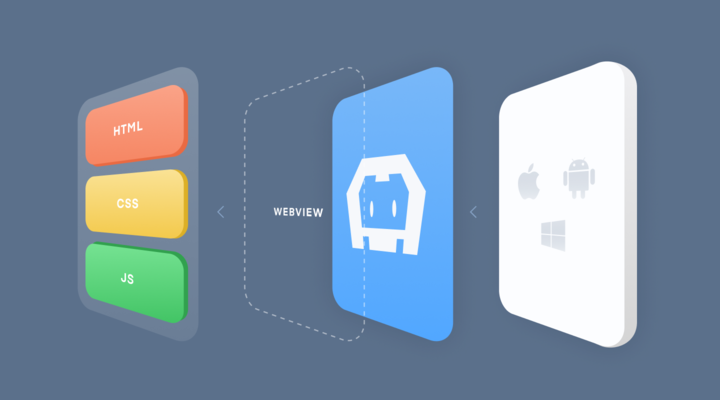
\includegraphics[scale=0.80]{img/cap2/cordova}\\

Apache Cordova è un framework di sviluppo di applicazioni mobili che può essere utilizzato per creare app mobili multipiattaforma usando HTML5 e puro JavaScript. 
Per multipiattaforma, intendiamo che il codice di applicazione può essere scritto una volta utilizzando HTML5 e JavaScript e può essere eseguito su diversi OS; come Android, iOS o Windows Mobile.

Riporto qua un frammento di codice che permette di aprire la camera nativa del dispositivo mobile.

\begin{lstlisting}
ionic cordova plugin add cordova-plugin-camera
npm install @ionic-native/camera
\end{lstlisting}

\begin{lstlisting}
import { Camera, CameraOptions } from '@ionic-native/camera/ngx';

const options: CameraOptions = {
  quality: 100,
  destinationType: this.camera.DestinationType.FILE_URI,
  encodingType: this.camera.EncodingType.JPEG,
  mediaType: this.camera.MediaType.PICTURE
}

constructor(private camera: Camera) { }

openCamera(){
    this.camera.getPicture(options).then((imageData) => {
        // imageData is either a base64 encoded string or a file URI
        // If it's base64 (DATA_URL):
        let base64Image = 'data:image/jpeg;base64,' + imageData;
        }, (err) => {
        // Handle error
    });
}
\end{lstlisting}

Vediamo come in 16 linee di codice siamo riusciti a raggiungere il seguente risultato, sia su IOS che su Android:

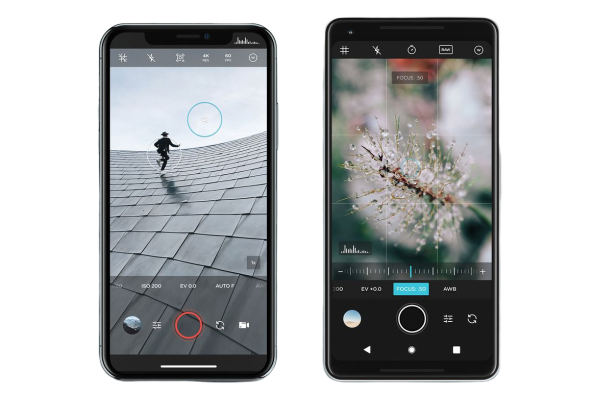
\includegraphics[scale=0.60]{img/cap2/camera}


\paragraph{}
\textit{SASS}

Scrivere CSS (Cascading Style Sheets) è fondamentale per descrivere in modo efficace il modo in cui gli elementi HTML devono 
essere visualizzati su una pagina Web per definire stili, design, layout e tutto ciò che è necessario per creare un sito 
Web sbalorditivo. Ma quando inizi a lavorare con siti grandi e complessi, potresti iniziare a chiederti se i CSS potrebbero 
essere migliori. 

In questi casi entra in gioco SASS (Syntacticly Awesome Stylesheets).
SASS è un pre-processore CSS che consente di utilizzare variabili, operazioni matematiche, mixin, loop, funzioni, importazioni 
e altre funzionalità interessanti che rendono la scrittura CSS molto più potente. In un certo senso, si potrebbe pensare a 
SASS come a un linguaggio di estensione del foglio di stile perché estende le caratteristiche CSS standard introducendo i
vantaggi di un linguaggio di programmazione di base. Quindi SASS compilerà il codice e genererà l'output CSS che un
browser può comprendere.

\paragraph{}
\paragraph{}
\paragraph{}
\paragraph{}

Vediamo alcune funzioni SASS in confronto con CSS puro:\\

\textit{Variabili}
\begin{multicols}{2}
    \begin{lstlisting}
// SASS
$font-stack:    Helvetica, sans-serif
$primary-color: #333

body
    font: 100% $font-stack
    color: $primary-color
    \end{lstlisting}
    \columnbreak
    \begin{lstlisting}
// CSS
body {
    font: 100% Helvetica, sans-serif;
    color: #333;
} 

.
    \end{lstlisting}
\end{multicols}

\begin{multicols}{2}
    \columnbreak
\end{multicols}


\textit{Mixin}

\begin{multicols}{2}
    \begin{lstlisting}
// SASS
@mixin transform($property) 
    -webkit-transform: $property
    -ms-transform: $property
    transform: $property

.box
    @include transform(rotate(30deg))   
    \end{lstlisting}
    \columnbreak
    \begin{lstlisting}
// CSS
.box {
    -webkit-transform: rotate(30deg);
    -ms-transform: rotate(30deg);
    transform: rotate(30deg);
}

.
    \end{lstlisting}
\end{multicols}

\paragraph{}
\paragraph{}
\paragraph{}
\paragraph{}
\paragraph{}
\paragraph{}
\paragraph{}

\textit{Loop}


\begin{multicols}{2}
    \begin{lstlisting}
// SASS
$class-slug: for !default

@for $i from 1 through 4
    .#{$class-slug}-#{$i}
    width: 60px + $i









    .
    \end{lstlisting}

    \columnbreak
    \begin{lstlisting}
// CSS
.for-1 {
    width: 61px;
}

.for-2 {
    width: 62px;
}

.for-3 {
    width: 63px;
}

.for-4 {
    width: 64px;
}
    \end{lstlisting}   
\end{multicols}
   

\subsection{NgRx gestore stato}
\paragraph{}
NGRX è un gruppo di librerie per Angular ispirate al pattern Flux sviluppato dal team di Facebook per gestire
lo stato delle applicazioni client.

Lo scopo principale di questo pattern è fornire uno stato dell'applicazione prevedibile, basato su tre principi principali.

\begin{itemize}
    \item \textbf{Unica sorgente di verità}: significa che l'intero stato dell'applicazione è memorizzato nella
    stessa struttura dati.
    \item \textbf{Lo stato è read only}: lo stato non viene mai cambiato direttamente, 
    solo tramite \textit{action}. Le \textit{action} descrivono cosa sta succedendo (possiamo vedere le action
    come richieste di ottenimento dati, rimozione, aggiornamento stato).
    \item \textbf{I cambiamenti sono fatti solo da funzioni pure}: quando un' \textit{action} viene lanciata, essa verrà
    intercettata dai \textit{reducer}.
    Questi \textit{reducer} (sono solo funzioni pure) ricevono un'azione e lo stato, a seconda dell'azione inviata 
    (di solito con un'istruzione switch) eseguono un'operazione e restituiscono un nuovo oggetto di stato. 
    Lo stato in un'app redux è immutabile! Quindi, quando un \textit{reducer} modifica qualcosa nello stato, 
    restituisce un nuovo oggetto stato.
\end{itemize}

\paragraph{}
\begin{figure}[h!]
    \centering  
    \caption{NgRx flow}
    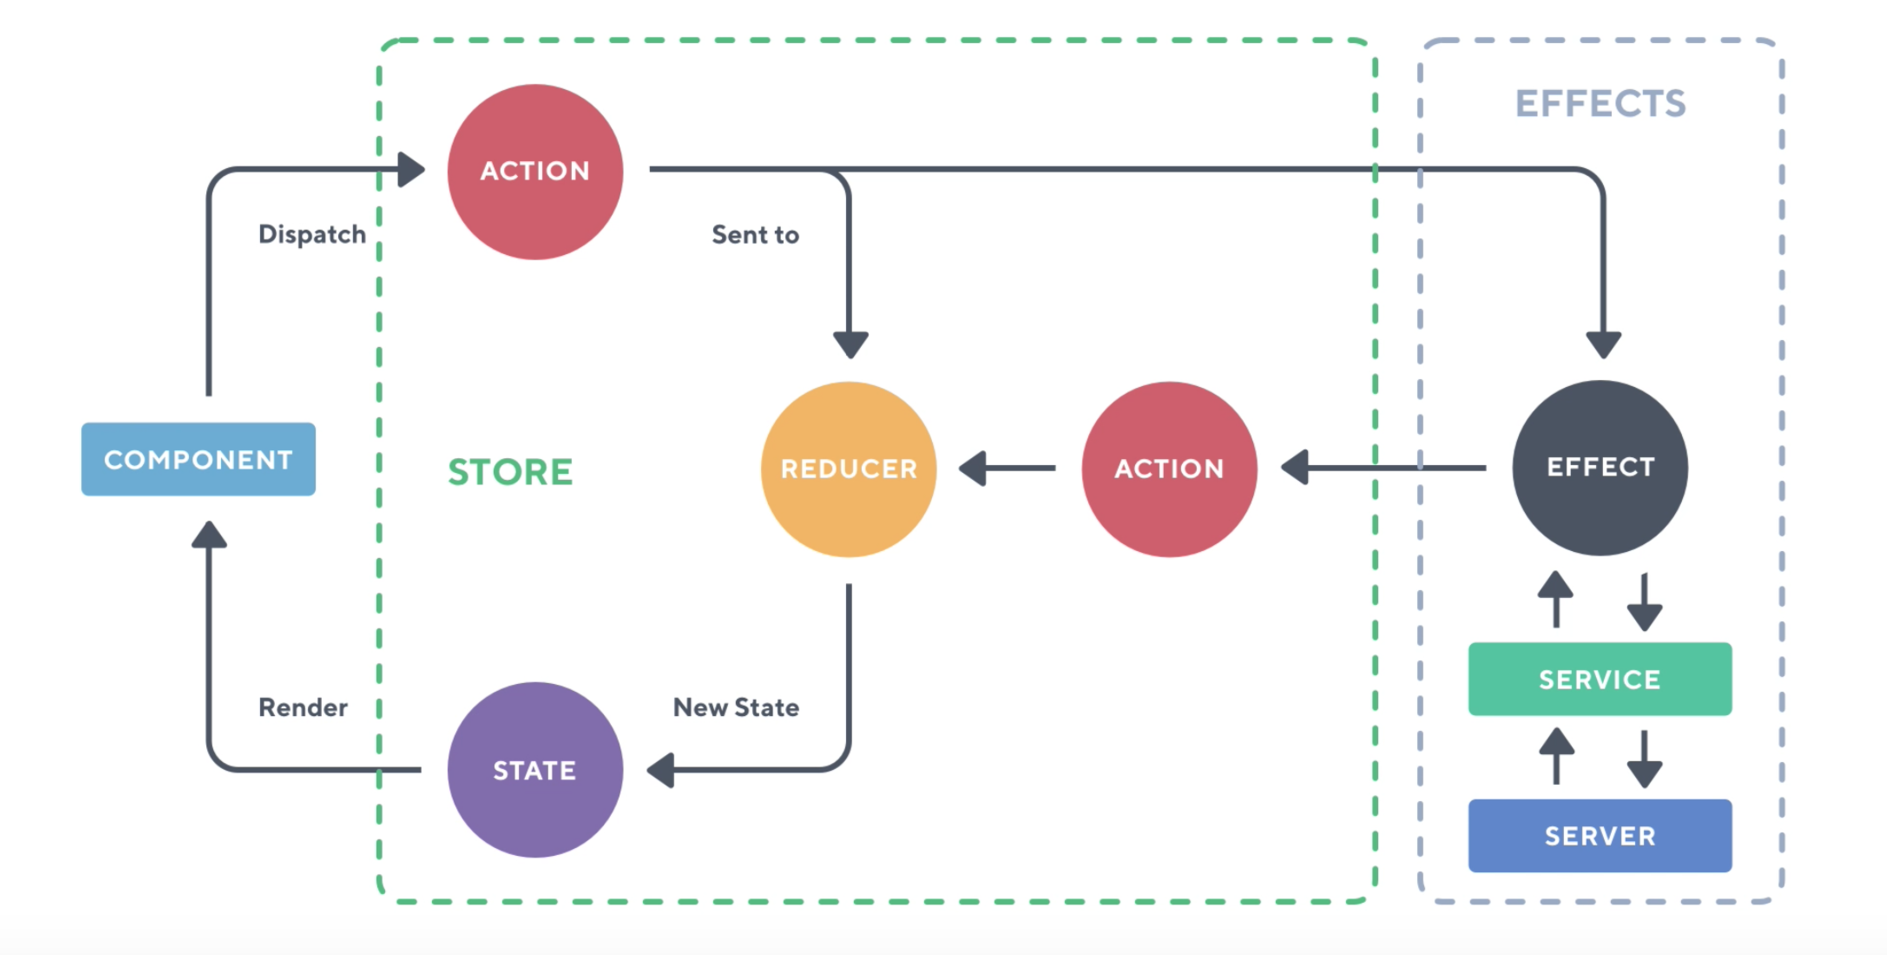
\includegraphics[scale=0.4]{img/cap2/ngrx}
\end{figure}
\paragraph{}

\begin{figure}[h!]
    \centering  
    \caption{Without NgRx}
    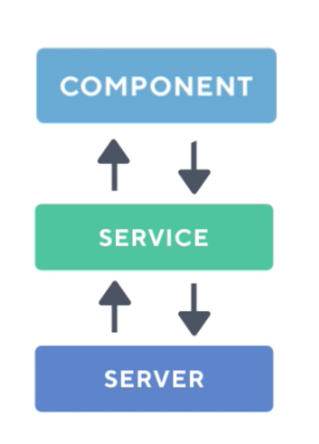
\includegraphics[scale=0.5]{img/cap2/without-ngrx}
\end{figure}
\paragraph{}

\begin{figure}[h!]
    \centering  
    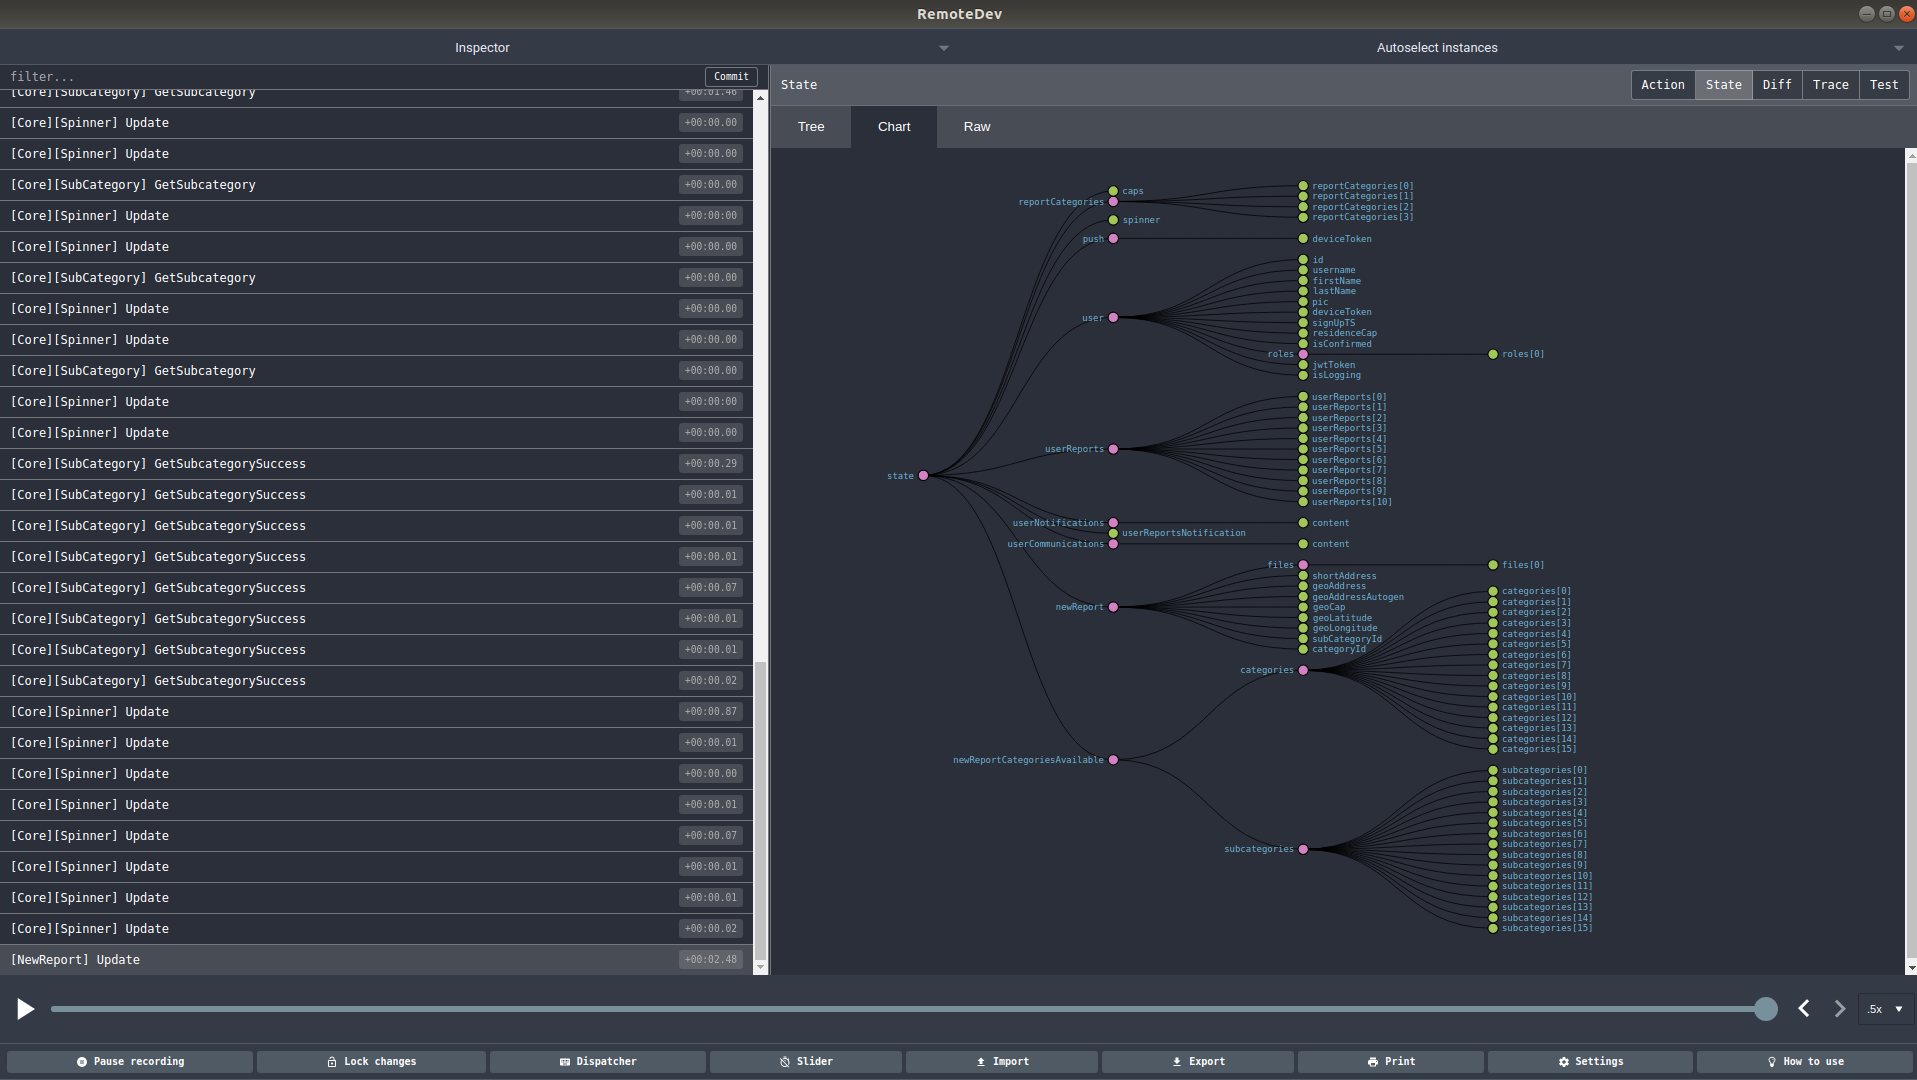
\includegraphics[scale=0.2]{img/cap2/ngrx-eservant}
\end{figure}

\section{Social login}
Al primo accesso all'APP eServant è necessario dare il consenso per almeno uno dei seguenti social:
\begin{itemize}
\item Facebook
\item Instagram
\item Twitter
\end{itemize}

Altrimenti viene data la possibilità di fare un accesso privato tramite username e password.
L'autenticazione verso i social network sopra citati avviene tramite protocollo OAuth2.0.

Il framework di autorizzazione OAuth 2.0 abilita un'applicazione di terze parti a ottenere un accesso limitato a un servizio HTTP, attivo
per conto di un proprietario di risorse orchestrando un'inerazione di approvazione tra il proprietario della risorsa e il servizio HTTP.
Questa specifica sostituisce e obsoleta il protocollo OAuth 1.0 descritto in RFC 5849.
\paragraph{}
\paragraph{}
\paragraph{}

OAuth 2.0 flow 

\begin{figure}[h!]
    \centering  
    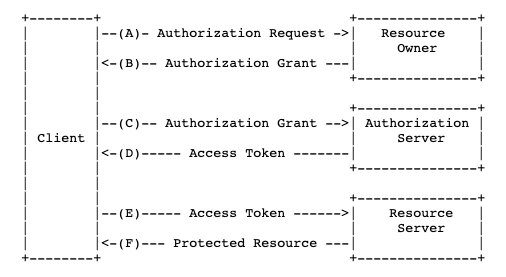
\includegraphics[scale=0.60]{img/cap2/oauth20-1}
\end{figure}

\paragraph{}

\textbf{Attori}

\begin{itemize}
\item \textit{resource owner}: un'entità in grado di approvare l'accesso a una risorsa protetta.
\item \textit{authorization server}: il server che invia i token di accesso al client dopo essere stato autorizzato
dal resource owner
\item \textit{resource server}: il server che ospita le risorse protette. Il resource Server è in grado di accettare
e rispondere alle richieste di risorse protette utilizzando i token di accesso.
\item \textit{client}: un'applicazione che fa richieste di risorse protette per conto di
proprietario di risorse e con la sua autorizzazione. Il termine "client"
non implica particolari caratsteristiche di implementazione (l'applicazione può essere eseguita
su un server, un client web o altri dispositivi).
\end{itemize}


\section{Navigazione impianto}
Grazie alla collaborazione con il MICC di Firenze siamo riusciti ad integrare una cartografia basata su OpenStreetMap
per permettere ai partecipanti di eventi la navigazione verso un determinato POI (point of interest) partendo
dall'ultima posizione rilevata del partecipante.

Il nostro compito si è suddiviso in tre parti:
\begin{itemize}
\item Creazione livelli da applicare alle mappe OSM per la navigazione interna
\item Integrazione delle mappe sia sull'APP Ionic che sul backoffice web
\item Recupero ultima posizione dell'utente
\end{itemize}

Visto che questa feature di eServant è un software standalone, l'integrazione all'interno dell'app Ionic è stata fatta
tramite iframe.
Frammento di codice:
\begin{lstlisting}[language=html]
<iframe src="https://www.eservant.it/maps"></iframe>
\end{lstlisting}

\paragraph{}

\begin{figure}[htp]
    \centering  
    \subfloat[Selezione POI]{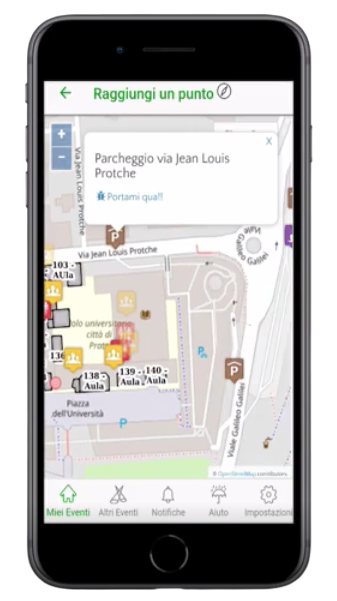
\includegraphics[scale=0.5]{img/cap2/maps-1}}
    \subfloat[Avvio navigazione verso il POI]{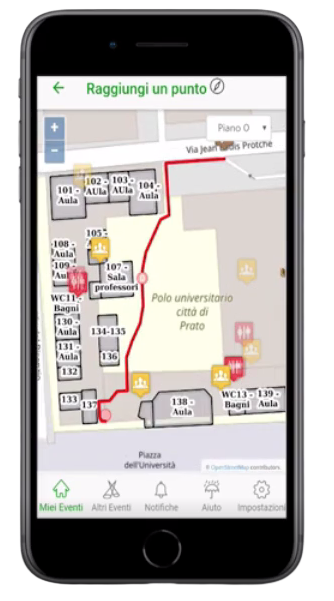
\includegraphics[scale=0.5]{img/cap2/maps-2}}
\end{figure}


\section{Geolocalizzazione}
Come ho detto nella sezione precedente, la navigazione all'interno dell'impianto necessità la posizione iniziale
dalla quale far iniziare il percorso verso il POI selezionato.
Questa posizione ovviamente è un elemento dinamico che deve mutarsi nel tempo dipendentemente dalla posizione
dell'utente all'interno dell'impianto.

Da un primissimo brainstorming è emerso che la tecnologia GPS non è affidabile in impianti indoor ma anche in ambienti
outdoor potrebbe fallire; per questo principale motivo è stata creata una gerarchia di tecnologie da usare per
la Geolocalizzazione dell'utente, dalla più affidabile alla meno affidabile.

In ordine di priorità di affidabilità decrescente, troviamo:

\begin{itemize}
    \item QRcode manuale
    \item GPS
    \item iBeacon
\end{itemize}


Risultato finale:
\begin{figure}[H]
    \centering  
    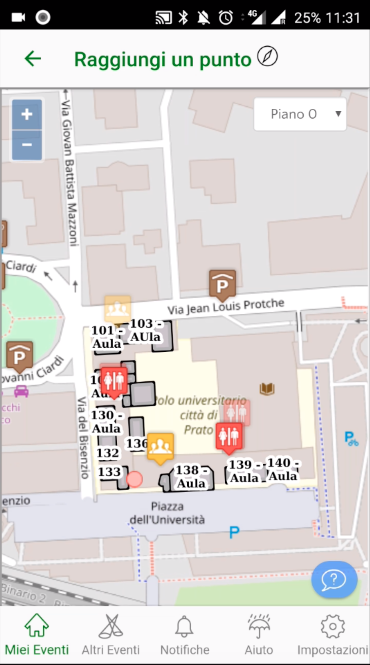
\includegraphics[scale=0.5]{img/cap2/geo-1}
\end{figure}


\subsection{QRcode}
\begin{figure}[H]
    \centering  
    
\includegraphics[scale=1]{img/cap2/barcode-qrcode}
\end{figure}
I codici QR sono stati creati nel 1994 da Denso Wave, una filiale giapponese del Gruppo Toyota.
L'uso di questa tecnologia è ora gratuito. Il QR Code non è l'unico codice a barre bidimensionale 
sul mercato, un altro esempio è il codice Data Matrix.
\\
Un codice QR è un codice a barre quadrato bidimensionale che può memorizzare dati codificati. 
Il più delle volte i dati sono un link a un sito web (URL).

Nel caso di eServant il codice QRcode racchiude un identificativo di un POI. \\
Vediamo le fasi del processo di geolocalizzazione tramite QRcode:

\begin{enumerate}
    \item Scansione QRcode tramite l'app di eServant
    \item Decodifica del QRcode e ottenimento del POI ID
    \item Invio del POI ID, insieme all' ID dell'utente, al server
    \item Il server, una volta ottenute le coordinate del POI, provvede ad aggiornare l'ultima posizione dell'utente
\end{enumerate}

\begin{lstlisting}
import { BarcodeScanner } from '@ionic-native/barcode-scanner/ngx';

constructor(private barcodeScanner: BarcodeScanner) { }

this.barcodeScanner.scan().then(barcodeData => {
    console.log('Barcode data', barcodeData);
}).catch(err => {
    console.log('Error', err);
});
\end{lstlisting}

\subsection{GPS}

\begin{figure}[H]
    \centering  
    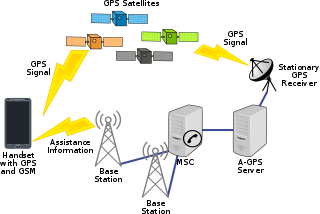
\includegraphics[scale=0.6]{img/cap2/gps}
\end{figure}

\begin{lstlisting}
import { Geolocation } from '@ionic-native/geolocation/ngx';

constructor(private geolocation: Geolocation) {}

this.geolocation.getCurrentPosition().then((resp) => {
    // resp.coords.latitude
    // resp.coords.longitude
}).catch((error) => {
    console.log('Error getting location', error);
});

let watch = this.geolocation.watchPosition();
watch.subscribe((data) => {
    // data can be a set of coordinates, or an error (if an error occurred).
    // data.coords.latitude
    // data.coords.longitude
});
\end{lstlisting}

\subsection{iBeacon}

\begin{figure}[H]
    \centering  
    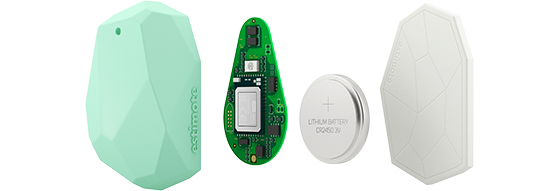
\includegraphics[scale=0.3]{img/cap2/beacon}
\end{figure}

iBeacon è una tecnologia basata su Bluetooth Low Energy. A partire dal 2013 iBeacon è 
integrato in Apple iOS 7. Il primo progetto pilota è stato lanciato nei negozi Apple nel
Dicembre 2013.

\textbf{BLE (Bluetooth Low Energy)}
Bluetooth Low Energy (BLE) è uno standard di trasmissione radio sviluppato dalla community 
Bluetooth SIG. Le caratteristiche di questo standard sono mirate a soddisfare le esigenze
delle moderne applicazioni wireless, come un consumo energetico estremamente basso, una
connessione corta che scandisce i tempi, affidabilità e sicurezza. 
BLE consuma da 10 a 20 volte meno energia (e 1000 volte meno del Wi-Fi), e può trasmettere
dati con velocità 50 volte superiore rispetto al Bluetooth classico. 

Lato client (Ionic), il plugin cordova IBeacon mette a disposizione due principali metodi
che permettono di intercettare due eventi:

\begin{itemize}
    \item Dispositivo mobile entrato nel raggio dell'ibeacon
    \item Dispositivo mobile uscito dal raggio dell'ibeacon
\end{itemize}

\begin{figure}[H]
    \centering  
    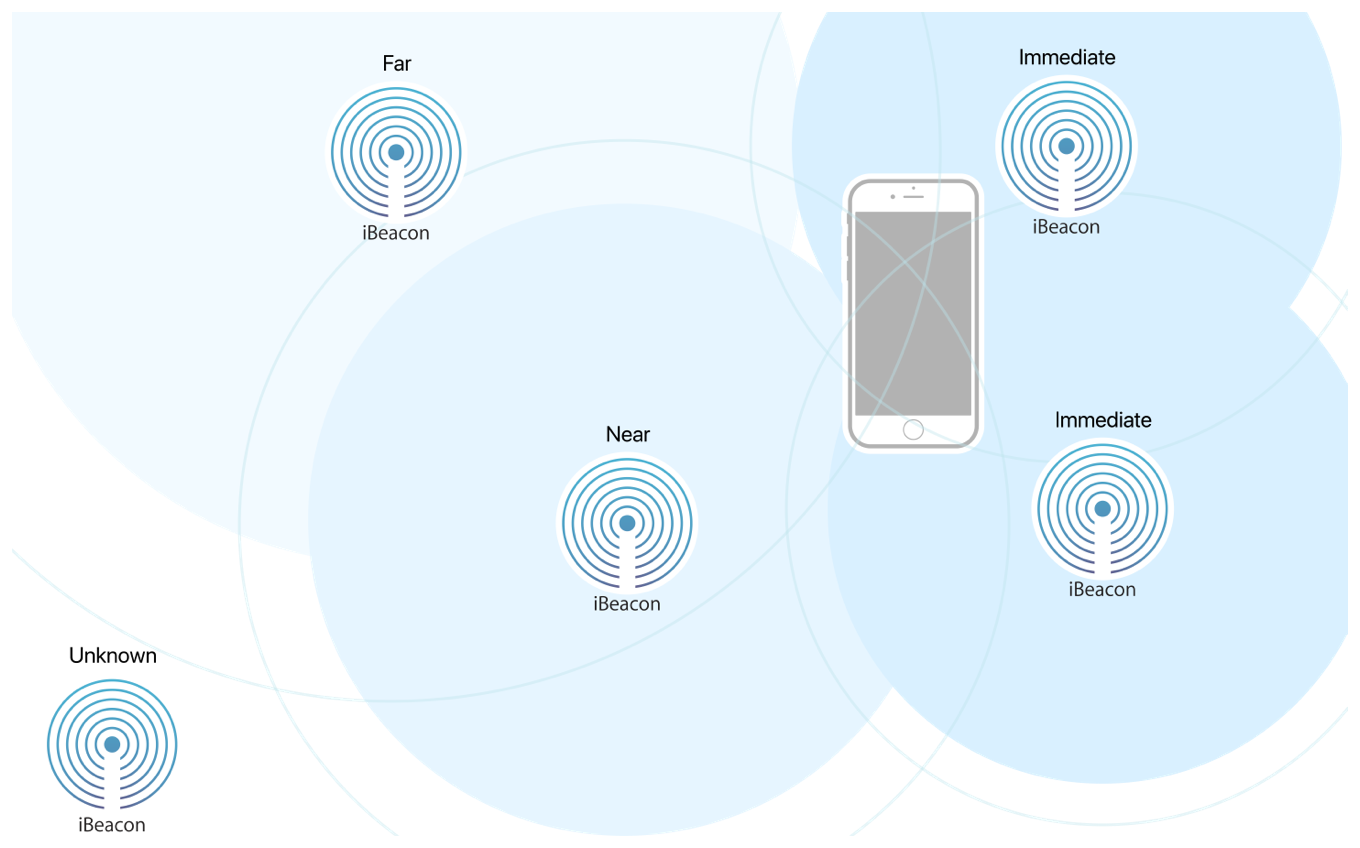
\includegraphics[scale=0.3]{img/cap2/beacon-proximity}
\end{figure}


Frammento di codice Ionic:
\begin{lstlisting}
import { IBeacon } from '@ionic-native/ibeacon/ngx';

constructor(private ibeacon: IBeacon) { }

// create a new delegate and register it with the native layer
let delegate = this.ibeacon.Delegate();

// Subscribe to some of the delegate's event handlers
delegate.didRangeBeaconsInRegion()
  .subscribe(
    data => console.log('didRangeBeaconsInRegion: ', data),
    error => console.error()
  );
delegate.didStartMonitoringForRegion()
  .subscribe(
    data => console.log('didStartMonitoringForRegion: ', data),
    error => console.error()
  );
delegate.didEnterRegion()
  .subscribe(
    data => {
      console.log('didEnterRegion: ', data);
    }
  );

let beaconRegion = this.ibeacon.BeaconRegion('deskBeacon','F7826DA6-ASDF-ASDF-8024-BC5B71E0893E');

this.ibeacon.startMonitoringForRegion(beaconRegion)
  .then(
    () => console.log('Native layer received the request to monitoring'),
    error => console.error('Native layer failed to begin monitoring: ', error)
  );
\end{lstlisting}

\section{Chatbot}

Il chatbot agisce come supporto automatico che, tramite una chat integrata nell'applicazione, cerca di rispondere
alle domande dell'utilizzatore.
Il motore dietro alla chat integrata è un NLP engine (Natural Language Processor).
Il suo compito è, per ogni stringa di testo proveniente dalla chat integrata sull'app, cercare di capire
il significato semantico della frase.

Introduciamo 2 concetti principali su cui si basa il motore NLP:

\begin{itemize}
\item Intent: rappresenta l'azione presente nella frase elaborata, è generalmente un verbo.
\item Slot: rappresenta uno o più attributi che si legano all'intent. In molti casi l'intent è lo stesso,
cambiano solo i valori degli slot.
\end{itemize}

Vediamo nel caso specifico di eServant.

\begin{figure}[htp]
    \centering  
    \subfloat[Domanda]{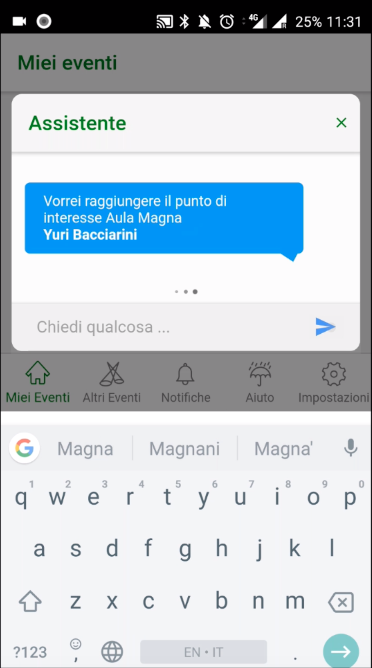
\includegraphics[scale=0.5]{img/cap2/chatbot-1}}
    \subfloat[Risposta]{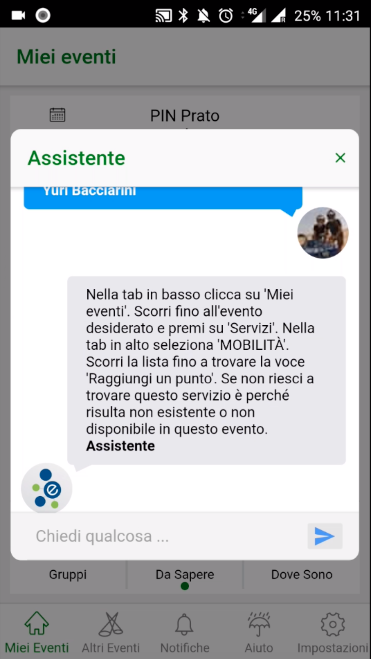
\includegraphics[scale=0.5]{img/cap2/chatbot-2}}
\end{figure}

\textit{Vorrei \textcolor{green}{raggiungere il punto di interesse} \textcolor{purple}{Aula Magna}}\\
Analisi tramite NLP:
\begin{itemize}
\item \textbf{intent}: \textcolor{green}{raggiungere il punto di interesse}
\item \textbf{slot}: 
\begin{itemize}
    \item Tipo slot: POI
    \item Valore: \textcolor{purple}{Aula Magna}
\end{itemize}
\end{itemize}
    
\subsection{Brainstorming}
\begin{figure}[htp]
    \centering  
    \subfloat[Brainstorming]{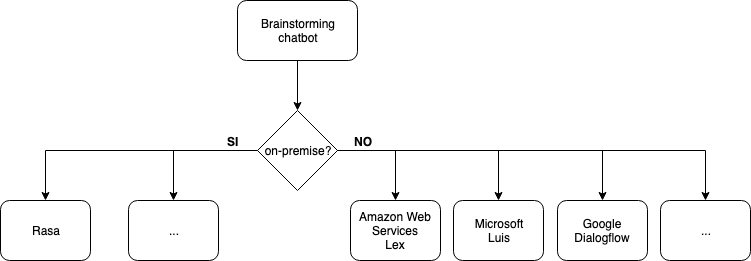
\includegraphics[scale=0.5]{img/cap2/eservant-chatbot}}
\end{figure}


Come si nota dal flow decisionale, la prima domanda che ci siamo posti è stata se volevamo fare il deploy del
chatbot su cloud oppure in-house.\\

Vediamo nel dettaglio le differenze principali tra le due strade:\\
\textbf{Cloud}\\
\textit{pro}\\
\begin{itemize}
    \item servizio pronto all'uso
    \item semplice da configurare, allenare, mantenere
    \item riceve aggiornamente continui
    \item scalabilità
\end{itemize}
\textit{contro}
\begin{itemize}
    \item costo non basso (generalmente per singola chiamata)
    \item privacy, i dati vengono trasmetti sui server del cloud provider
    \item non portabile
\end{itemize}
\paragraph{}

\textbf{In-house}\\
\textit{pro}\\
\begin{itemize}
    \item privacy, i dati non escono dalla workstation
    \item controllo del provider infrastrutturale
\end{itemize}
\textit{contro}
\begin{itemize}
    \item tempi di apprendimento e sviluppo maggiori
    \item mantenimento
\end{itemize}

\subsection{implementazione}

\begin{figure}[htp]
    \centering  
    \subfloat[Flow di decisione]{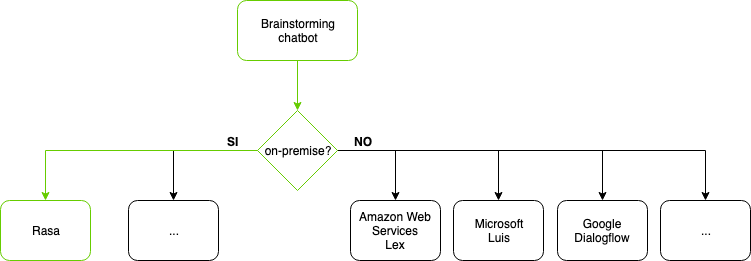
\includegraphics[scale=0.5]{img/cap2/eservant-chatbot-green}}
\end{figure}

Visto che il progetto eServant racchiude informazioni private degli impianti, abbiamo deciso di usare un motore
NLP in-house e non cloud.
Date le conoscenze in Quid Informatica del linguaggio di programmazione Python abbiamo deciso di procedere
con l'implementazione del chatbot usando il framework Rasa, scritto appunto in Python.

Rasa è un framework open source in Python per la creazione di chatbot basato su machine learning.
Invece che basarsi su una cascata di if/else, Rasa risponde usando un modello, creato attraverso
librerie di machine learning in Python sulla base di conversazioni campione.
